
\section{Occupational Choice and Knowledge Diffusion}\label{section:theory}

In this section, we build on  the theory of  accumulation and dissemination of knowledge through the combination of ideas (\citeNP{kortum1997research}, \citeNP{lucas2009}, \citeNP{lucas2014}). We add to this theory a new occupational choice, which can be biased by the presence of censorship.
Authors, building on the knowledge created by the previous generation, write books that can be compliant with the Catholic Church's ideology or revolutionary (in the sense of the Humanistic and Scientific Revolutions). Printers decide whether to be active in the revolutionary or compliant sector. They make this choice according to the quality of the books of each type that they encounter.  The Catholic Church dislikes revolutionary ideas and might decide to censor them. This would decrease the share of revolutionary books, and hence their quality, redirecting printers towards compliant books. This distortion  alters the accumulation of the total stock of knowledge in the economy.

\subsubsection*{Knowledge Diffusion}

Time is discrete. At each date $t$ one generation of $S$ persons is alive. Knowledge is embodied in books and is transmitted between the successive generations through them. At the beginning of each period, the individuals first learn from $\mu_t$ books. $\mu_t$ is a parameter representing the number of books one can buy during her life. We let it depend on time to allow changes in $\mu_t$, for example when income or length of life changes.  Books include more or less relevant content to produce goods and services. A book  $i$ has a characteristic $h_i$ drawn from an exponential distribution. $h_{i}$ should be seen as a negative feature, for example the irrelevance of the book. The quality of a book is a decreasing function of its irrelevance, with elasticity $\theta$:
\begin{equation}\label{eq:qi}
q_i=h_i^{-\theta}, \;\;\; \theta\in(0,1).
\end{equation}
Books are of two types, which define different distributions from which their relevance is drawn. \textit{Compliant} books, indicated by the superscript ${C}$, embody the type of knowledge that is compliant with the ideology of the Catholic Church.
%\footnote{Note that being compliant does not necessarily mean to produce work using the official Catholic Church doctrine as an input: this is true just for the production of religious books or religious services in general. %Instead, it just means that the knowledge should not contradict the Catholic Church doctrine.}
\textit{Revolutionary} books, denoted by the superscript $R$, contain knowledge that is considered heretical by the Catholic Church. Taking examples from \citeN{alexander2014infinitesimal}, geometry books would be compliant while books using infinitesimal calculus would be revolutionary. Both of them are of variable quality, which we call relevance. At the beginning of time $t$, the irrelevance of book $i$ of type $j$ follows an exponential distribution
\begin{equation}
h^j_i \sim \exp(k_{t}^j), \quad \text{with} \ j\in \{C,R\}.
\end{equation}
Note that the scale parameter $k_{t}^j$ depends on the book type.
As the expected value of $h^j_i$ equals the inverse of $k^j_{t}$, $k^j_{t}$ measures the average usefulness of knowledge in sector $j$.


Since the irrelevance of books is exponentially distributed and given Equation~(\ref{eq:qi}), the distribution of book quality follows a Fr\'echet distribution, see Appendix~\ref{O-app:frechet}.   The distribution of book quality represents the technology frontier. The median ($Q_2(q^j)$) and third quartile $(Q_3(q^j))$ of book quality, used in the estimation, are:
%\begin{equation}
%E(q^j_i)=\Gamma(1-\theta) \; (k^j)^{\theta} \text{with} \ j\in \{C,R\},
%\end{equation}
\begin{equation}
Q_2(q^j) = (k^j)^{\theta} [\log(2)]^{-\theta}, \;\;\; Q_3(q^j)=	(k^j)^{\theta} [\log(4/3)]^{-\theta} \;\;\; \text{with} \ j\in \{C,R\}.
\end{equation}



The number of revolutionary books that each agent will read in $t+1$ depends on their availability in bookshops. The share of printers that produced revolutionary books in the previous generation is denoted by  $m_{t}$. Therefore, a individual will read $\lfloor \mu_{t+1} m_{t} \rfloor$ revolutionary books  and $\lfloor \mu_{t+1} (1-m_{t}) \rfloor$ compliant books, drawn from their respective distribution. Each individual $s$ retains the best book coming from each one of the two distributions.
 Formally, the process of retaining the best books by sector is described as
\begin{align*}	
   \hat{h}^C_s&=\text{min}\{h^C_1,..,h^C_{\lfloor(1-m_{t}) \mu_{t+1}\rfloor}\},
 \\ \hat{h}^R_s&=\text{min}\{h^R_1,..,h^R_{\lfloor m_{t} \mu_{t+1} \rfloor}\}.
 \end{align*}
 For the sake of simplicity, from now on we will approximate $\lfloor(1-m_{t}) \mu_{t+1}\rfloor$ and $\lfloor m_{t} \mu_{t+1} \rfloor$ to respectively  $(1-m_{t})\mu_{t+1}$ and $m_{t} \mu_{t+1} $, so that we will be able to proceed with our analysis treating the number of books read as a continuous variable.
As the exponential distribution satisfies the minimum stability postulate, we have:
\begin{align*}
\min\{h^C_1,..,h^C_{(1-m_{t}) \mu_{t+1}}\}& \sim \exp(k^C_{t} (1-m_{t}) \mu_{t+1}),\;\;\;\mbox{ and }\\
\min\{h^R_1,..,h^R_{ m_{t} \mu_{t+1} }\}& \sim \exp(k^R_{t} m_{t} \mu_{t+1}).
 \end{align*}
Hence, the distribution of actual relevance of the best book read by person $s$ follows
\begin{equation}
 \hat{h}^j_s \sim \exp(b_{t+1}^j), \quad \text{with} \ j\in \{C,R\},
\end{equation}
where $b_{t+1}^C$ and $b_{t+1}^R$ are defined as
 \begin{align*}
  b_{t+1}^C&=k_{t}^C (1-m_{t}) \mu_{t+1}, \\
  b_{t+1}^R&=k_{t}^R m_{t}  \mu_{t+1}.
 \end{align*}

Later in life, the generation $t+1$ writes new books,  combining their inherited knowledge with a new idea. This new idea is drawn from a distribution whose scale parameter depends on the average quality of the books they have read:
$$
h^j_{sN}\sim  \exp(\nu b^j_{t+1}), \quad \text{with} \ j\in \{C,R\}.
$$
Taking the best of their acquired and new knowledge leads to a book with irrelevance distributed as:
\begin{equation}
\tilde h^j_s=\min(h^j_{sN},\hat h^j_s) \sim  \exp((1+\nu) b^j_{t+1}). \label{eq:writing}
\end{equation}
We can now summarize the dynamics of the two types of knowledge by the dynamics of the scale of their distribution:
 \begin{align}
  k_{t+1}^C&=(1+\nu) k_{t}^C (1-m_{t}) \mu_{t+1},\label{eq:kCtime} \\
  k_{t+1}^R&=(1+\nu) k_{t}^R m_{t} \mu_{t+1}. \label{eq:kRtime}
 \end{align}


 \subsubsection*{Occupational Choice}

We now define how the share of printers producing revolutionary books evolves over time. We suppose that printers have to decide whether to be active in the compliant sector or in the revolutionary sector at the beginning of their activity. Once they have chosen a sector, they would print any author they meet randomly.
They will thus determine their sector of activity based on the first author $s$ they meet. This author has written two book projects of relevance $\tilde{h}^C_s$ and $\tilde{h}^R_s $. Only one of these two book projects will be printed: the printed book will have quality $q^C_i$ or $q^R_i$, according to which book project was chosen. There are $2S$ book projects, which reduces to $S$ books actually printed. Printers decide their sector taking into account the relative relevance of the two books. Printers also take into account that customers of the bookshop might value differently two books with the same quality that belong to two different sectors. This might happen because of consumer preferences or because of the way in which book quality translates into consumption goods.
%\footnote{Books can be used to produce consumption goods, and books belonging to different sectors can have different productivity in this respect. For example, the production of consumption goods through books can be %represented as $c=\alpha\sum^{N_R} q_i^R+\sum^{N_C} q_i^C$, where $\alpha$ would be the relative productivity of revolutionary books' quality, while $N_R$ and $N_C$ are respectively the number of revolutionary and compliant %books owed by the customer.}
We summarize these two effects assuming that the relative price at which revolutionary books are sold is represented by $p$.  Using the properties of the exponential distribution (see Appendix~\ref{O-app:oc_ch}), we can write a closed form expression for the probability that the revolutionary book is best:
\begin{equation}
\text{Prob}\{q^C_i<p q^R_i\}=\text{Prob}\{\tilde{h}^C_s>p^{-1/\theta}\tilde{h}^R_s\}=\frac{b^R_{t+1}}{b^R_{t+1}+b^C_{t+1} p^{-1/\theta}}=m_{t+1}.\label{eq:occupation}
\end{equation}
Using the law of large numbers, this probability also defines the share of printers active in the revolutionary sector $m_{t+1}$. From now on we will refer to $\hat{p}$ as $\hat{p}=p^{-1/\theta}$.

Since $k^j_{t+1}=(1+\nu)b^j_{t+1}$, Equation~(\ref{eq:occupation}) can be we written as
\begin{equation}\label{eq:sharer}
m_{t+1}=\frac{k^R_{t+1}}{k^R_{t+1}+\hat{p}k^C_{t+1}}.
\end{equation}
The dynamics of knowledge quality (\ref{eq:kCtime}) and (\ref{eq:kRtime}),  together with the occupation choice (\ref{eq:sharer})
and initial conditions $k_{1}^C$ and $k_{1}^R$, determine $m_{1}$ and the equilibrium path $\{ m_t,  k_{t}^C,  k_{t}^R\}_{t\geq 1}$.


\subsubsection*{Censorship}\label{subsection:censor}

So far, the Church did not play any role in the model. We now let  the Church interfere with the process of occupational choice imposing a rate of censorship on revolutionary books. More precisely, she can limit the number of revolutionary titles that an author can read, making unavailable a fraction $\beta$ of the volumes that she would have read without censorship. Formally, the process of censorship limits the number of revolutionary books that individuals in $t+1$ encounter during their life to $\mu_{t+1} m_t (1-\beta)$ and therefore alters the process of accumulation of revolutionary knowledge, which now follows
\begin{equation}\label{eq:censorhip}
k_{t+1}^R=(1+\nu)(1-\beta)k_{t}^R m_{t} \mu_{t+1}, \quad\text{with} \ \beta\in[0,1].
\end{equation}
Note that in this way, the Church can decrease the current share of revolutionary books $m$ and %will
also make it less likely that revolutionary works will be written in the future. This is because the accumulation of revolutionary knowledge slows down. The law of motion of $k_{t+1}^C$ (see Equation~(\ref{eq:kRtime})) does not change when the Church imposes censorship on revolutionary books.


The Church could also limit the spread of revolutionary books by persecuting authors and printers accused of heresy. This fact matters for the accumulation of knowledge as authors and printers might decide to self-censor their works to avoid risk to their life. The baseline model does not feature self-censorship, but we include this mechanism in a robustness check in Appendix~\ref{O-app:robust}.



\subsubsection*{The Dynamics under an Exogenous Church's Behavior}\label{sec:exo}

So far we mentioned that the Church can limit the share of revolutionary books through censorship, but we did not mention how the Church is choosing $\beta$. Clearly, the choice of  $\beta$ over time will depend on the behavior of agents described in the previous section and on the objective of the Catholic Church. On the one hand, the Church wanted to have the smallest possible number of heretical books circulating, to maintain its power. On the other hand, we do not know what prevented the Church from imposing the highest level of censorship in any period. The Church was probably trading off censorship with other motivations. It could have been because the Church was directing attention elsewhere, or because overly harsh censorship could create damage to the Church itself,\footnote{As an example, we can think that if the censorship is overly harsh, the Catholic Church might lose in terms of competition with the Protestant Church. This reasoning is plausible if devotees dislike censorship that is too harsh. While rulers had the final say about the religion of their territory, their decision was not completely independent from the common people's beliefs. Protestantism could spread thanks to the invention of the printing press, which aroused popular support by distributing pamphlets \cite{eisenstein1980,rubin2014}. Probably it would not be the best choice for a ruler to impose Catholicism if a large majority of the population already had converted to Protestantism.} or something else.

Here we treat $\beta$ as if it was exogenous, and we study the dynamics under this assumption. We start defining $z=k^R/k^C$: note that the share or revolutionary ideas $m$ can assume one and only one value given $z$, which means that once we know the dynamics of one of the two variables, we also know the dynamics of the other. From equation (\ref{eq:sharer}) we get
\begin{equation}\label{eq:sharer2}
m_t=\frac{z_t}{\hat{p}+z_t}.
\end{equation}
 We decided to make $m_t$ rather than $z_t$ our main variable for describing the model dynamics because its domain is a bounded set.
% The dynamics of $m$ are defined formally below.
%\begin{definition}\label{definition:equilibrium}
%	Given a censorship rate $\beta$,  an exogenous process $\{\mu_t\}_{t>1}$, and initial conditions on  knowledge quality in the compliant and revolutionary sectors    %$k_{1}^C$ and $k_{1}^R$,  an equilibrium path is a sequence $\{ m_t,  k_{t}^C,  k_{t}^R\}_{t\geq 1}$, describing the share of revolutionary books and knowledge quality %in both sectors over time. In equilibrium, it is such that:
%	\begin{itemize}
%	\item Each author of  generations $t>1$ writes book projects whose quality and type is defined by combining acquired and new knowledge according to %(\ref{eq:writing}).
%	\item Each printer of  generations $t\geq 1$ chooses her sector according to the most productive book presented by the first randomly met author, i.e. following %(\ref{eq:occupation}). Each printer of each generation, once she chooses her sector, prints all the authors she meets randomly.
%	\item For all $t\geq 1$, the probability of being exposed to revolutionary book in $t+1$  depends on the share of revolutionary titles written in $t$. The books %printed in $t$ embody the stock of compliant and revolutionary knowledge available to generation $t+1$. Knowledge quality in the compliant and revolutionary sectors %evolves according to (\ref{eq:kCtime})-(\ref{eq:kRtime}).
%	\end{itemize}
%\end{definition}
The equilibrium  can be summarized in a single equation by the law that governs the dynamics of $m$.
Dividing Equation~(\ref{eq:censorhip}) by (\ref{eq:kCtime}) side by side, and substituting the resulting $z_{t+1}$ in (\ref{eq:sharer2}) at time $t+1$, we get the equation that governs the equilibrium dynamics of $m$:
\begin{equation}
m_{t+1}=\frac{(1-\beta) m_t^2}{1-m_t ((\beta -2) m_t+2)}=f(m_t;\beta)\label{eq:lawm}.
\end{equation}
Equation~(\ref{eq:lawm}) and an initial  $m_1$, allow us to determine the equilibrium path $\{m_t\}_{t\geq1}$. The initial $m_1$ depends on the initial conditions we have imposed and on parameter $\hat{p}$  through:
$$m_1=
\frac{k^R_1}{k^R_1+\hat{p}k^C_1}
$$
The equilibrium path $\{m_t\}_{t\geq1}$  satisfies:
\begin{proposition}
	Given the initial $m_1\in[0,1)$, the long run share of revolutionary authors, $m\equiv\lim_{t\to\infty}m_t$, is given by
	\begin{itemize}[itemsep=1mm, parsep=0pt,topsep=0pt]
    \item[i)]$m=0$ if $m_1<1/(2-\beta)$ (Compliant steady state),
    \item[ii)] $m=1$ if $m_1>1/(2-\beta)$ (Revolutionary steady state),
     \item[iii)]$m=m_1$ if $m_1=1/(2-\beta)$ (Unstable steady state).
	\end{itemize}
	 \label{proposition:dynex}
\end{proposition}
\begin{proof}See Appendix~\ref{O-app:prf1}\end{proof}


\begin{figure}
\begin{center}
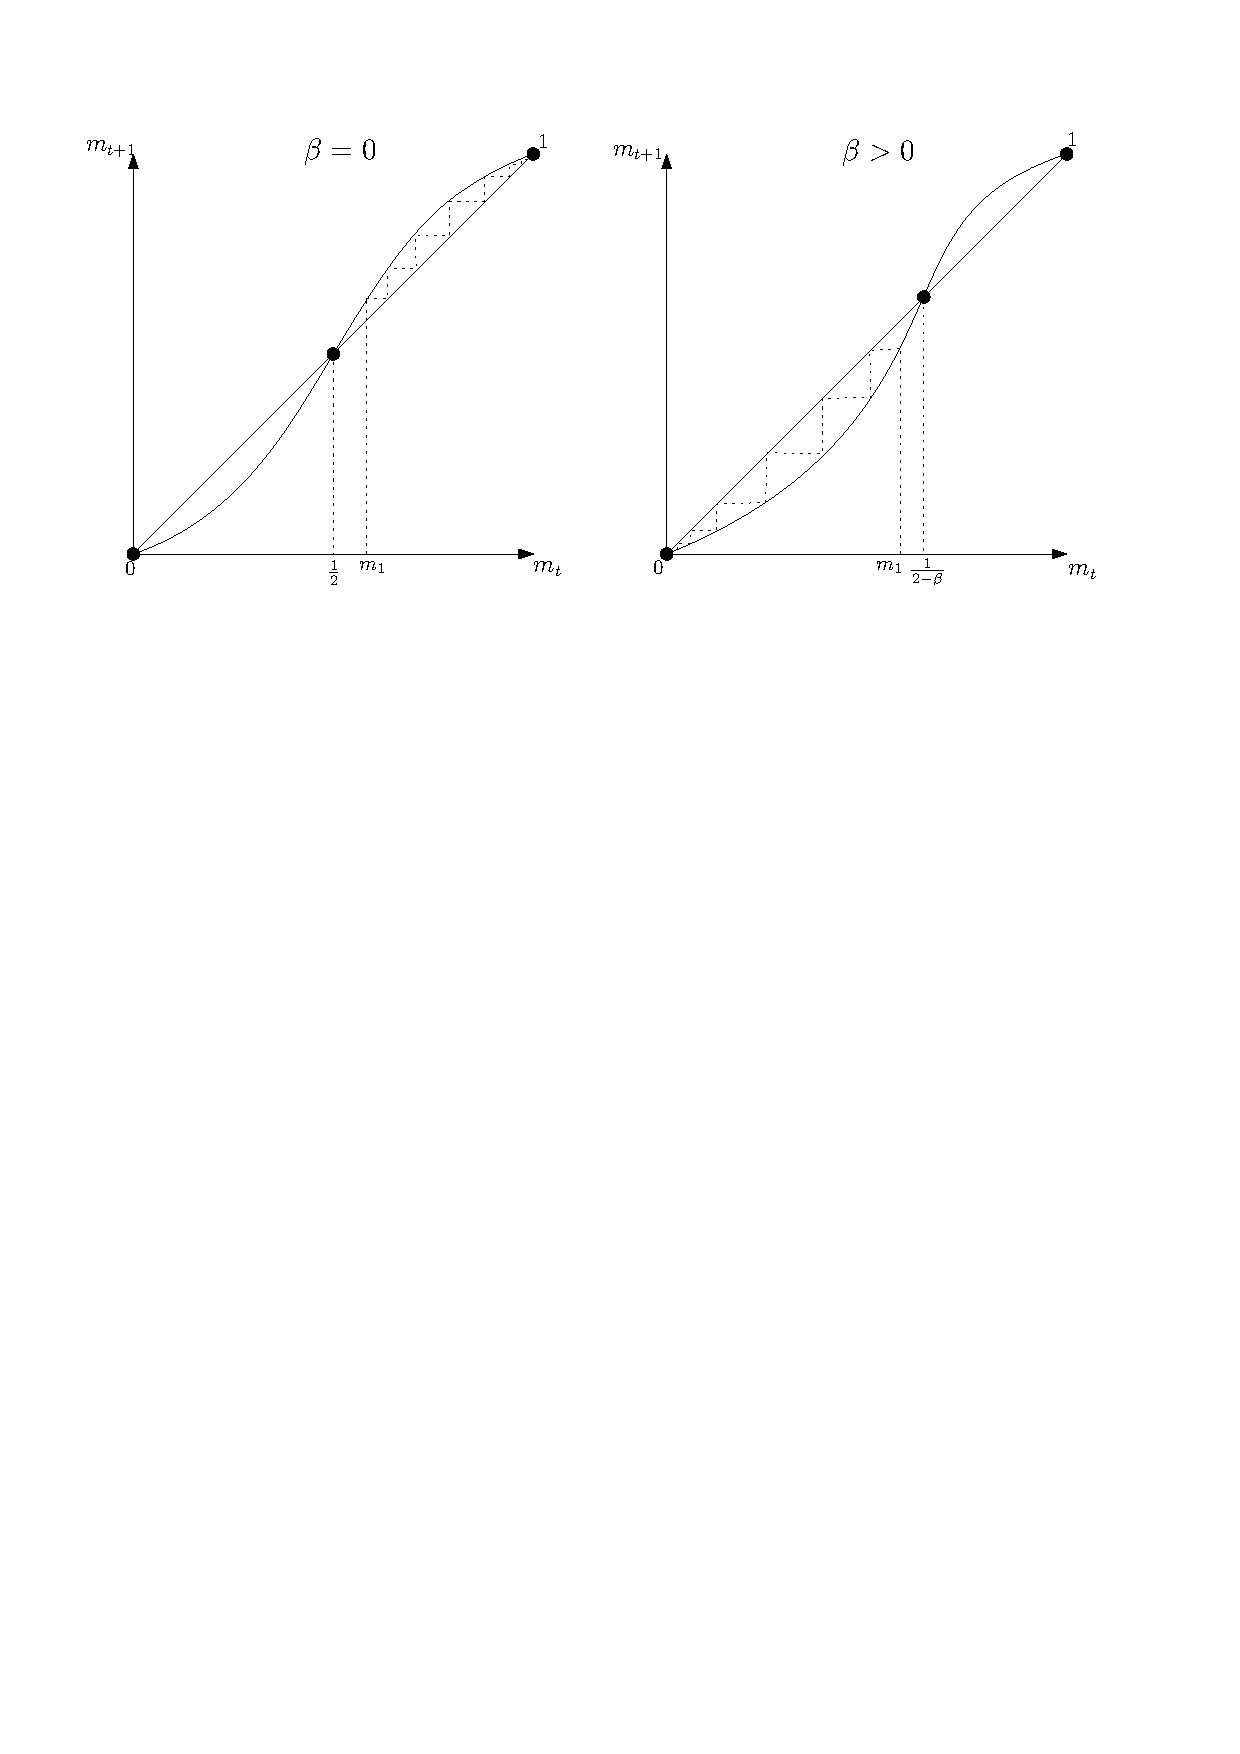
\includegraphics[width=15cm]{dynamics-m.pdf}
\end{center}
\caption{Dynamics of $m_t$ under no censorship (left) and exogenous censorship $\beta>0$ (right)}\label{fig:dynamics}
\end{figure}

Figure~\ref{fig:dynamics} illustrates Proposition~\ref{proposition:dynex}. On the left, there is no censorship. The two locally stable steady states are 0 and 1. Their basin of attraction is delimited by the unstable steady state $1/2$. On the right, there is a positive censorship rate. The dynamic function is shifted to the right, and the unstable steady state delimiting the two basins of attraction is larger and equal to $1/(2-\beta)$. The figure depicts a situation in which, for the same initial condition $m_1$, dynamics converge to the Revolutionary steady state under no censorship $\beta=0$, but to the Compliant steady state with $\beta>0$.

Notice that the path of $m_t$ does not depend on the process $\mu_t$, but quality levels $k^R_t$ and $k^C_t$ do.


\subsubsection*{The Dynamics under an Optimizing Church's Behavior}

In the previous subsection, we described the dynamics under a constant rate of censorship $\beta_t$. A simple way to go beyond this approach would be to assume a rule of thumb behavior of the type: the Church chooses the lowest rate of censorship that allows convergence to a world with no revolutionary ideas. We analyzed this case in Appendix~\ref{O-app:thumb}.
This approach has two main shortcomings. Firstly, it makes strong assumptions regarding how the Church trades off the gains and losses of imposing censorship. Secondly, it leaves unexplained the timing of censorship. Here we propose a model that can endogenize the timing of censorship and, most importantly, can explain the  features of authors' censorship that we illustrated in Section \ref{section:twof}. We assume that setting up an apparatus capable of creating a list of forbidden books and enforcing its application represented a large fixed cost for the Church. The Church cannot enforce any censorship before having paid a fixed cost $\psi$. After having paid $\psi$, she can impose a rate of censorship up to $\overline{\beta}$.

The maximum rate of censorship $\overline{\beta}<1$ depends on feasibility but also on political economy considerations.
Italy was not a unified state, but was divided into multiple states with their own objectives and relationships with the Church/Papal States. In the presence of a more or less unified market for books, the Church, to be effective in its censorship, had to avoid making too unhappy any of the Italian states, which could have otherwise decided to play the role of heresy-spreader by protecting local authors and publishers from persecution. This placed a constraint on the Church ability to censor.

The Church cares about the share of compliant books in the economy: its utility function is given by $u()$, which is differentiable, bounded, and strictly increasing in $1-m_t$. We write this problem recursively in Appendix~\ref{O-app:recursive}.

In Appendix~\ref{O-app:recursive} we also show that when $m_1$ is large or small enough, the convergence forces to the steady state dominate the benefits of imposing censorship. Thus, in these cases, setting up a (costly) censorship apparatus is not optimal.  Whether it is optimal to impose censorship for intermediate $m_1$ depends on the model parameters, which we estimate in the next section.

